\documentclass[11pt]{article}

\usepackage[T1]{fontenc}
\usepackage[utf8]{inputenc}
\usepackage{amsmath,amssymb,amsfonts}
\usepackage{graphicx}
\usepackage{bm}
\usepackage{siunitx}
\usepackage{geometry}
\usepackage[colorlinks=true,linkcolor=black,citecolor=blue,urlcolor=blue]{hyperref}
\usepackage[noabbrev,nameinlink]{cleveref}
\geometry{margin=1in}

\title{Self-starting Siphon Priming: Geometry, Limits, Analytics, and Computation}
\author{Stelios Raptopoulos}
\date{20 November 2025}

\begin{document}
\maketitle

\begin{abstract}
Self-starting siphons use a deliberate drop in the centreline to generate a momentum-bearing water slug that climbs a crest without external priming. This paper reconnects the full narrative: (i) a physical start-up description with explicit initial conditions, (ii) an exact container volume map for arbitrary internal pipe layouts (piecewise $h_c(L)$) and a constant-area simplification, (iii) modelling limits (cavitation head margin, capillarity, and non-hydrostatic inlet correction), (iv) a detailed filling-phase momentum balance with losses, and (v) an analytic upper bound on the maximum crest height reachable in the idealised lossless, fixed-$h_c$ case, expressed directly in terms of the piecewise-linear geometry. A complete Python integration script is provided to evolve the two-phase ODE system with Churchill friction, minor losses, events, and optional cavitation flagging.
\end{abstract}

\tableofcontents

\section{Introduction and mental model}
Self-starting siphons differ from a simple inverted-U siphon because the driving head remains non-zero while the front is above the container level but below the next crossing. An initial drop from $A$ to $B$ converts potential energy into kinetic energy; the momentum carries the slug upward until friction and gravity dissipate it. If the front crosses the crest at $D$, the pipe fills and the system drains like a conventional siphon.

The aims here are to (a) state clear initial conditions matching the physical start-up, (b) expose validity limits (cavitation, capillarity, non-hydrostatic inlet), (c) give an exact volume map for complex internal pipe paths and its constant-area specialisation, (d) retain the detailed loss derivation, and (e) provide both an analytic priming bound and a simulation recipe.
At the slug-model level developed below, the net force from pressure and gravity on the wetted portion is simply $\rho g A\bigl[h_c(t)-h(L)\bigr]$ (see \eqref{eq:Fdrive}). This term remains non-zero whenever the front elevation $h(L)$ lies below the container free surface $h_c$, so after the drop from $A$ to $B$ and into $BC$ the slug typically re-crosses the container level with finite velocity before decelerating towards the crest. In a simple inverted-U siphon the driving head vanishes at the crest after the initial drop, so the contrast in priming behaviour follows directly from this force term. The two experimental wetting procedures described in \cref{sec:initial} therefore collapse to the same slug-level initial state $t_0=0$, $L(0)=L_1$, $\dot L(0)=0$, $h_c(0)=h_0$.

Self-starting siphons and priming behaviour have been discussed in the literature; see Potter and Barnes~\cite{potter_barnes}, Jumper and Stanchev~\cite{jumper_stanchev}, Zheng et al.~\cite{zheng_siphon}, Ortloff and Kassinos~\cite{ortloff_kassinos}, and Sedlar et al.~\cite{sedlar_siphon}. Cavitation limits are treated in \cite{boatwright,vera,tyree}. Losses follow Churchill \cite{churchill} and standard handbooks \cite{crane,colebrook,moody,white}.

\section{Geometry and coordinate systems}
\label{sec:geometry}

\subsection{Global coordinates and centreline}
We work in a vertical $(x,h)$ plane with $h$ measured upward from the container base. Five node points define the centreline:
\[
  A(0,h_0),\quad B(x_1,h_1),\quad C(x_2,h_2),\quad D(x_3,h_3),\quad E(x_4,h_4),
\]
connected by straight segments of lengths
\begin{align*}
  L_1 &= \sqrt{(x_1-0)^2 + (h_1-h_0)^2}, &
  L_2 &= \sqrt{(x_2-x_1)^2 + (h_2-h_1)^2},\\
  L_3 &= \sqrt{(x_3-x_2)^2 + (h_3-h_2)^2}, &
  L_4 &= \sqrt{(x_4-x_3)^2 + (h_4-h_3)^2}.
\end{align*}
The total length is $L_{\max}=L_1+L_2+L_3+L_4$, with cumulative arclengths $S_0=0$, $S_1=L_1$, $S_2=L_1+L_2$, $S_3=L_1+L_2+L_3$, $S_4=L_{\max}$.

The piecewise-linear elevation is
\[
h(L)=
\begin{cases}
  h_0 + \dfrac{L}{L_1}(h_1-h_0), & 0\le L\le L_1,\\[0.8em]
  h_1 + \dfrac{L-L_1}{L_2}(h_2-h_1), & L_1\le L\le L_1+L_2,\\[0.8em]
  h_2 + \dfrac{L-L_1-L_2}{L_3}(h_3-h_2), & L_1+L_2\le L\le L_1+L_2+L_3,\\[0.8em]
  h_3 + \dfrac{L-L_1-L_2-L_3}{L_4}(h_4-h_3), & L_1+L_2+L_3\le L\le L_{\max}.
\end{cases}
\]
On segment $i$ (spanning $[S_{i-1},S_i]$) it is convenient to write
\begin{equation}
  h(L) = c_i + s_i L,\qquad
  s_i = \frac{h_i-h_{i-1}}{L_i},\qquad
  c_i = h_{i-1} - s_i S_{i-1}.
  \label{eq:linear-hi}
\end{equation}
If segment $i$ makes an angle $\theta_i$ with the horizontal, then $s_i=\sin\theta_i$, so only the vertical projection of each leg enters the climb analysis.

\begin{figure}[htbp]
  \centering
  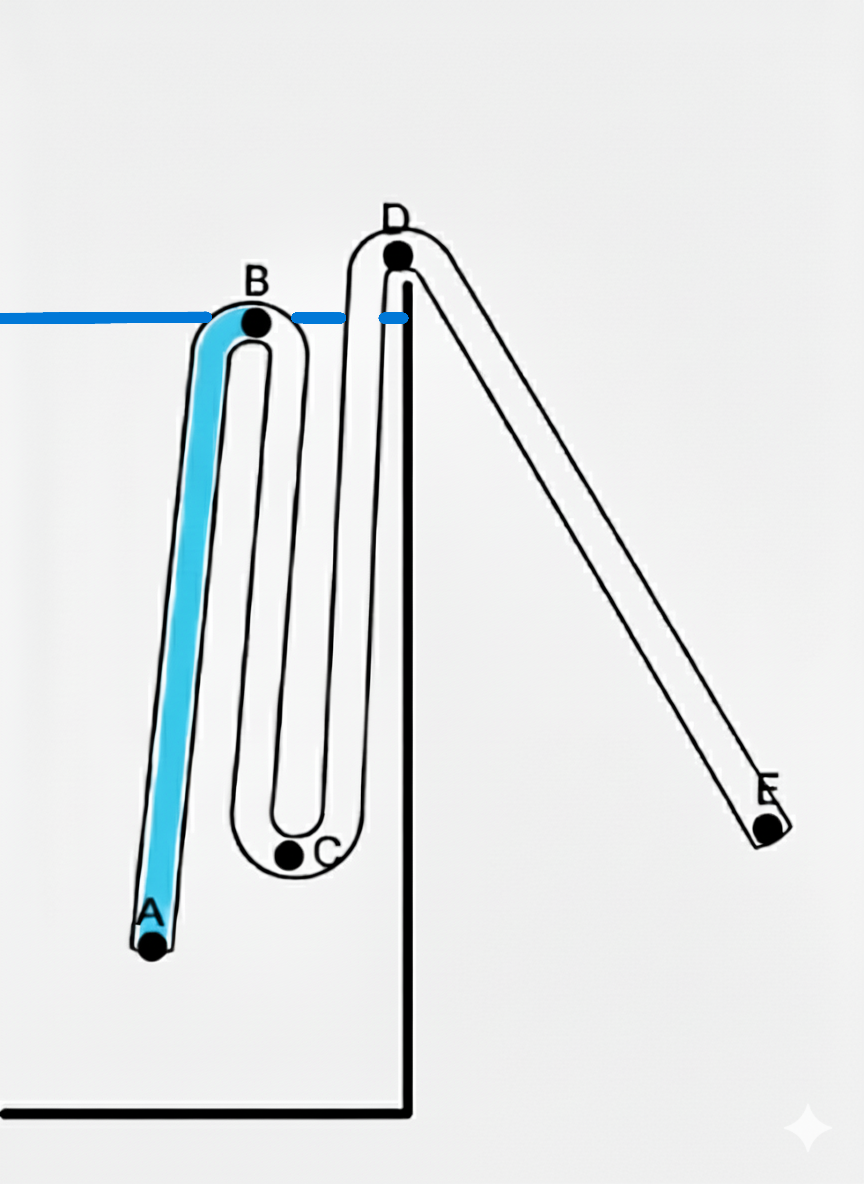
\includegraphics[width=0.82\textwidth]{siphon_diagram.png}
  \caption{Self-starting siphon geometry and notation. Points $A$--$E$ define the centreline, $h(L)$ is the piecewise elevation, and $h_c$ is the container free surface.}
\end{figure}

\subsection{Wetted length $L(t)$}
During filling, the wetted length $L(t)$ tracks the water--air interface along the centreline. Its elevation is $h_{\text{front}}(t)=h(L(t))$. When $L(t)=L_{\max}$ the pipe is full.

\section{Container, volume map, and effective area}
\label{sec:container}
Let $A$ be the pipe cross-section (diameter $D$). The container cross-sectional area available to water at height $\eta$ is $A_{\mathrm{eff}}(\eta)=A_{\mathrm{cyl}}-n(\eta)A$, where $n(\eta)$ counts pipe legs intersecting that slice. The exact container volume up to $h_c$ is
\begin{equation}
  F(h_c) = \int_0^{h_c} A_{\mathrm{eff}}(\eta)\,d\eta.
  \label{eq:F-def}
\end{equation}
In the filling phase no water exits, so total volume is conserved:
\begin{equation}
  F(h_c(t)) + A L(t) = F(h_0) + A L_1.
  \label{eq:global-volume}
\end{equation}
This is exact for any internal layout. Note that $F(h)$ is the container water volume excluding the pipe interior, because $A_{\mathrm{eff}}$ subtracts the cross-sectional area of each leg that intersects the slice. Inverting gives $h_c(L)=F^{-1}(F(h_0)+A(L_1-L))$; for piecewise-constant $n(\eta)$, $h_c(L)$ is piecewise linear with slope changes where $n(\eta)$ jumps. For a concrete geometry, $n(\eta)$ is obtained by listing the heights at which pipe segments enter or leave the container and counting how many legs are present on each interval, after which the integrals in \eqref{eq:F-def} are elementary.

\paragraph{Example of piecewise $n(\eta)$.} If $n(\eta)=0$ on $[0,h_a)$, $n(\eta)=1$ on $[h_a,h_b)$, and $n(\eta)=2$ on $[h_b,h_c)$, then
\[
F(h)=
\begin{cases}
  A_{\mathrm{cyl}} h, & 0\le h<h_a,\\
  A_{\mathrm{cyl}} h - A(h-h_a), & h_a\le h<h_b,\\
  A_{\mathrm{cyl}} h - A(h-h_a) - A(h-h_b), & h_b\le h<h_c,
\end{cases}
\]
so $h_c(L)$ is linear in each interval of $h$ with slope changes at $h_a,h_b$.

\subsection{Constant-area specialisation}
If the pipe footprint is small or effectively constant with height, take $A_{\mathrm{eff}}\approx A_0$ so $F(h)=A_0 h$ and \eqref{eq:global-volume} reduces to
\begin{equation}
  h_c(L) = h_0 - \frac{A}{A_0}(L-L_1).
  \label{eq:hc-L}
\end{equation}
The pipe interior volume is already counted by $AL$, even if portions lie below $h_c$.

\section{Validity limits and missing physics}
\label{sec:limits}
\begin{itemize}
  \item \textbf{Hydrostatic inlet assumption.} The inlet pressure is $p_{\mathrm{atm}}+\rho g(h_c-h_0)$. This is valid if the free surface moves slowly: $|\dot h_c|\ll \sqrt{gD}$ and $|\ddot h_c|\ll g$. Rapid drawdown adds an unsteady Bernoulli term; a crude correction to the driving head is an extra term of size $\Delta h_{\text{unsteady}}\approx -(A/A_0)\dot h_c\,\dot L/g$, which is small under the same inequalities.
  \item \textbf{Cavitation / tensile failure.} The minimum centreline pressure (often near the crest) must satisfy $p_{\min}\ge p_{\mathrm{vap}}$ (or the tensile limit in \cite{boatwright,vera,tyree}). A conservative head margin is
  \begin{equation}
    h_c - h_{\text{crest}} - h_{\text{loss,crest}} \ge h_{\mathrm{vap}},
    \qquad h_{\mathrm{vap}} = \frac{p_{\mathrm{atm}}-p_{\mathrm{vap}}}{\rho g}.
    \label{eq:cavitation}
  \end{equation}
  If \eqref{eq:cavitation} is violated, expect column separation.
  \item \textbf{Capillarity / meniscus.} For small $D$, start-up requires overcoming meniscus pressure. A threshold head $h_{\sigma}\approx 4\sigma\cos\theta/(\rho g D)$ (Jurin height) must be exceeded; once $v>0$ the standard loss model applies.
  \item \textbf{Slug-model limits.} Strong curvature, air entrainment, turbulent slug breakup, or three-dimensional paths invalidate the 1D slug model; such cases need two-phase or CFD treatment.
\end{itemize}

\section{Initial conditions and inverted-U contrast}
\label{sec:initial}
Two practical wetting methods yield the same dynamic start:
\begin{enumerate}
  \item \emph{Pre-fill to $B$.} Raise the free surface quasi-statically to $B$, fully wetting $AB$, then release.
  \item \emph{Dip to $B$.} Submerge the inlet so the interface reaches $B$, then place the leg in position.
\end{enumerate}
In both cases the wetted length tracks the free surface until the interface reaches $B$, giving
\begin{equation}
  t_0 = 0,\qquad L(0)=L_1,\qquad \dot L(0)=0,\qquad h_c(0)=h_0.
  \label{eq:IC}
\end{equation}
From there, the front drops into $BC$, gaining momentum from the non-zero driving term $\rho gA(h_c-h(L))$. In an inverted-U siphon the driving head vanishes at the crest after the initial drop; here it remains non-zero until the front rises back to the container level, so the slug typically crosses that level with finite speed unless losses are extreme.

\section{Dynamics in the filling phase}
\label{sec:filling}
Model the wetted portion as a slug of mass $m=\rho A L$ and mean velocity $v=\dot L$.

\subsection{Detailed lossless derivation}
Using a local coordinate $\xi$ along the pipe, the net tangential force on a slice combines the pressure gradient and gravity. Integrating from $\xi=0$ to $L$ yields
\[
  F_{\text{net}} = A\bigl[p(0,t)-p(L,t)\bigr] + \rho g A \bigl[h(0)-h(L)\bigr].
\]
Hydrostatic pressure at the inlet gives $p(0,t)=p_{\mathrm{atm}}+\rho g(h_c-h(0))$, while the outlet/front is at $p_{\mathrm{atm}}$, leading to the driving force
\begin{equation}
  F_{\text{drive}} = \rho g A\bigl[h_c(t) - h(L)\bigr].
  \label{eq:Fdrive}
\end{equation}
Newton's second law $m\ddot L = F_{\text{drive}}$ with $m=\rho A L$ gives the lossless equation
\begin{equation}
  \ddot L = \frac{g}{L}\bigl[h_c(t)-h(L)\bigr].
  \label{eq:filling-lossless-raw}
\end{equation}
With the constant-area map \eqref{eq:hc-L},
\begin{equation}
  \ddot L
  = \frac{g}{L}\Big[h_0 - \frac{A}{A_0}(L-L_1) - h(L)\Big].
  \label{eq:filling-lossless}
\end{equation}

\subsection{Loss models}
Distributed friction (Darcy--Weisbach) gives $h_f=f (L/D) v^2/(2g)$ with $f$ from Churchill \cite{churchill}:
\begin{align}
  \frac{f}{8} &= \left[\left(\frac{8}{\text{Re}}\right)^{12}
  + \frac{1}{(A_1 + A_2)^{3/2}}\right]^{1/12}, \label{eq:churchill-f} \\
  A_1 &= \left[-2.457 \ln\left(\left(\frac{7}{\text{Re}}\right)^{0.9}
  + 0.27\,\frac{\varepsilon}{D}\right)\right]^{16}, \label{eq:churchill-A1} \\
  A_2 &= \left(\frac{37530}{\text{Re}}\right)^{16}, \label{eq:churchill-A2}
\end{align}
with $\text{Re}=\rho |v|D/\mu$ and roughness $\varepsilon/D$. Minor losses add $K_i v^2/(2g)$; summing over elements gives $\sum_i K_i$.

The total loss head over wetted length $L$ is
\[
  h_{\text{loss}} = \Big(f\,\frac{L}{D}+\sum_i K_i\Big)\frac{v^2}{2g},
\]
corresponding to resistive force $\rho g A h_{\text{loss}}\operatorname{sgn}(v) = \tfrac{\rho A}{2}(f L/D + \sum_i K_i)|v|v$.

\subsection{Extended filling ODE}
Including losses, Newton's law becomes
\begin{equation}
  \ddot L
  = \frac{g}{L}\Big[h_0 - \frac{A}{A_0}(L-L_1) - h(L)\Big]
    - \frac{1}{2L}\Big(f\,\frac{L}{D} + \sum_i K_i\Big)|\dot L|\,\dot L.
  \label{eq:filling-extended}
\end{equation}
Integrate \eqref{eq:filling-extended} from \eqref{eq:IC} until $L(t^*)=L_{\max}$. The front height is $h_{\text{front}}=h(L(t))$.

\section{Idealised climb bound and analytical stall height}
\label{sec:bound}
Set $h_c\equiv h_0$, $f=0$, $\sum K_i=0$, and $\dot L(0)=0$ to obtain a geometry-only upper bound. Then
\begin{equation}
  \ddot L = \frac{g}{L}\bigl[h_0 - h(L)\bigr],\qquad \ddot L = v\,\frac{dv}{dL},\ v(L_1)=0,
  \label{eq:ideal-ddot}
\end{equation}
so
\begin{equation}
  v(L)^2 = 2g \int_{L_1}^{L} \frac{h_0 - h(\xi)}{\xi}\,d\xi.
  \label{eq:ideal-v2}
\end{equation}
The front stalls where $v(L_{\text{stall}})=0$, i.e.
\begin{equation}
  \int_{L_1}^{L_{\text{stall}}} \frac{h_0 - h(\xi)}{\xi}\,d\xi = 0,\qquad
  h_{\max}=h(L_{\text{stall}}).
  \label{eq:stall-condition}
\end{equation}

\subsection{Closed form for piecewise-linear $h(L)$}
On segment $i$, $h(L)=c_i+s_i L$; the segment contribution over $[a,b]\subseteq [S_{i-1},S_i]$ is
\begin{equation}
  \Phi_i(a,b) = (h_0-c_i)\ln\!\left(\frac{b}{a}\right) - s_i (b-a).
  \label{eq:Phi}
\end{equation}
For a candidate $L\in [S_{k-1},S_k]$,
\begin{equation}
  \sum_{i=2}^{k-1} \Phi_i(S_{i-1},S_i) + \Phi_k(S_{k-1},L) = 0
  \label{eq:stall-piecewise}
\end{equation}
is monotone in $L$ on that segment; solve it (e.g.\ bisection) to find $L_{\text{stall}}$ and $h_{\max}$. This is the analytic upper bound; drawdown and losses only decrease the reachable crest. A necessary geometric priming condition is
\begin{equation}
  h_{\max} > h_3,
  \label{eq:priming-criterion}
\end{equation}
because $D$ sits at elevation $h_3$.

\section{Dynamics in the draining phase}
\label{sec:drain}
When $L=L_{\max}$ the pipe is full; states are $h_c(t)$ and $v(t)$.

\subsection{Mass balance}
\begin{equation}
  \dot h_c = -\frac{A}{A_0} v.
  \label{eq:drain-mass}
\end{equation}

\subsection{Momentum with losses}
\begin{equation}
  L_{\max}\,\dot v
  = g(h_c - h_{\text{out}})
    - \frac{1}{2}\Big(f\,\frac{L_{\max}}{D} + \sum_i K_i\Big)|v|\,v,
  \label{eq:drain-mom}
\end{equation}
where $h_{\text{out}}=h(L_{\max})=h_4$. Initial conditions: $h_c(t^*)=h_0 - \tfrac{A}{A_0}(L_{\max}-L_1)$, $v(t^*)=\dot L(t^*)$. Neglecting inertia ($\dot v\approx 0$) yields the quasi-steady estimate
\begin{equation}
  v \approx \sqrt{\frac{2g(h_c-h_{\text{out}})}{f L_{\max}/D + \sum_i K_i}}.
  \label{eq:drain-quasi}
\end{equation}

\section{Computational approach (Python)}
\label{sec:comp}
Use event-driven integration: solve \eqref{eq:filling-extended} until $L=L_{\max}$, then switch to \eqref{eq:drain-mass}--\eqref{eq:drain-mom}. Recompute $f$ each step from \eqref{eq:churchill-f}--\eqref{eq:churchill-A2}; include $\sum K_i$ for the wetted length. An optional cavitation flag checks \eqref{eq:cavitation} along the centreline (evaluate $p=p_{\mathrm{atm}}+\rho g(h_c-h)-\rho g h_{\text{loss}}$).

\subsection*{Complete Python script}
\begin{verbatim}
import numpy as np
from math import log
from dataclasses import dataclass
from scipy.integrate import solve_ivp

def churchill_f(Re, eps_over_D):
    Re = max(Re, 1e-8)
    A1 = (-2.457*np.log((7/Re)**0.9 + 0.27*eps_over_D))**16
    A2 = (37530/Re)**16
    return 8 * (( (8/Re)**12 + 1.0/((A1 + A2)**1.5) )**(1/12))

@dataclass
class Params:
    g: float
    rho: float
    mu: float
    D: float
    A: float
    A0: float
    eps_over_D: float
    Ksum_fill: float
    Ksum_drain: float
    h0: float
    L1: float
    Lmax: float
    h_out: float
    # piecewise linear h(L)
    S: np.ndarray   # breakpoints [S0..S4]
    c: np.ndarray   # intercepts
    s: np.ndarray   # slopes

def h_of_L(L, p: Params):
    # find segment index
    idx = np.searchsorted(p.S, L, side='right') - 1
    idx = np.clip(idx, 0, len(p.S)-2)
    return p.c[idx] + p.s[idx]*L

def filling_rhs(t, y, p: Params):
    L, v = y
    h_c = p.h0 - (p.A/p.A0)*(L - p.L1)
    Re = p.rho*abs(v)*p.D/p.mu
    f = churchill_f(Re, p.eps_over_D)
    losses = f*L/p.D + p.Ksum_fill
    dvdt = (p.g/L)*(h_c - h_of_L(L,p)) - 0.5*(losses/L)*abs(v)*v
    return [v, dvdt]

def event_reach_outlet(t, y, p: Params):
    return y[0] - p.Lmax
event_reach_outlet.terminal = True
event_reach_outlet.direction = 1

def drain_rhs(t, y, p: Params):
    h_c, v = y
    Re = p.rho*abs(v)*p.D/p.mu
    f = churchill_f(Re, p.eps_over_D)
    losses = f*p.Lmax/p.D + p.Ksum_drain
    dvdt = (p.g/p.Lmax)*(h_c - p.h_out) - 0.5*(losses/p.Lmax)*abs(v)*v
    dhcdt = -(p.A/p.A0)*v
    return [dhcdt, dvdt]

# Example parameters (replace with experiment/geometry)
p = Params(
    g=9.81, rho=1000, mu=1e-3, D=0.01, A=np.pi*(0.01/2)**2,
    A0=0.02, eps_over_D=1e-4, Ksum_fill=1.0, Ksum_drain=1.0,
    h0=0.3, L1=0.05, Lmax=1.2, h_out=-0.4,
    S=np.array([0.0, 0.05, 0.55, 0.95, 1.2]),
    c=np.array([0.0, 0.05, -0.20, 0.10]),
    s=np.array([1.0, 0.5, 0.75, -1.0])
)

# Filling phase
y0 = [p.L1, 0.0]
sol_fill = solve_ivp(
    lambda t,y: filling_rhs(t,y,p),
    [0, 20], y0, rtol=1e-7, atol=1e-9,
    events=lambda t,y: event_reach_outlet(t,y,p)
)
L_end, v_end = sol_fill.y[0,-1], sol_fill.y[1,-1]
t_star = sol_fill.t_events[0][0]

# Draining phase
y0_drain = [p.h0 - (p.A/p.A0)*(p.Lmax - p.L1), v_end]
sol_drain = solve_ivp(
    lambda t,y: drain_rhs(t,y,p),
    [t_star, t_star+200], y0_drain, rtol=1e-7, atol=1e-9,
    events=lambda t,y: y[0] - p.h_out
)

print("Priming reached outlet at t* = %.4f s, L = %.3f, v = %.3f m/s"
      % (t_star, L_end, v_end))
if sol_drain.t_events[0].size:
    print("Draining stopped at t = %.2f s when h_c = h_out." %
          sol_drain.t_events[0][0])
\end{verbatim}
Adjust $p.S$, $p.c$, $p.s$ from \eqref{eq:linear-hi}, set $K$ values for fittings, and tighten tolerances if the flow is strongly damped. Add a cavitation check by evaluating $p_{\min}=p_{\mathrm{atm}}+\rho g(h_c-h_{\text{crest}})-\rho g h_{\text{loss,crest}}$ and flagging when it drops below $p_{\mathrm{vap}}$.

\section{Model summary}
\begin{itemize}
  \item Geometry: $h(L)$ piecewise linear via \eqref{eq:linear-hi}, $L_{\max}=S_4$, crest at $D$ with elevation $h_3$.
  \item Volume map: exact \eqref{eq:global-volume} with $F(h)$ from \eqref{eq:F-def}; constant-area map \eqref{eq:hc-L}.
  \item Filling: ODE \eqref{eq:filling-extended} with ICs \eqref{eq:IC}.
  \item Ideal bound: stall condition \eqref{eq:stall-piecewise}, $h_{\max}$, criterion \eqref{eq:priming-criterion}.
  \item Draining: \eqref{eq:drain-mass} and \eqref{eq:drain-mom}, quasi-steady \eqref{eq:drain-quasi}.
  \item Limits: cavitation margin \eqref{eq:cavitation}, capillary threshold $h_{\sigma}$, hydrostatic validity in \cref{sec:limits}.
\end{itemize}
\subsection*{Variables and parameters}
For quick reference, the main symbols are:
\begin{description}
  \item[$L(t)$] wetted length of the slug along the centreline, measured from $A$ to the water--air interface.
  \item[$h(L)$] centreline elevation at arclength $L$; see \eqref{eq:linear-hi}.
  \item[$h_c(t)$] container free-surface elevation measured from the container base.
  \item[$h_0$] initial container surface height, $h_c(0)$.
  \item[$v(t)$] mean slug velocity, $v=\dot L$.
  \item[$A$] pipe cross-sectional area (diameter $D$), $A=\pi D^2/4$.
  \item[$A_0$] effective container cross-sectional area in the constant-area model.
  \item[$L_{\max}$] total pipe length $S_4$.
  \item[$\rho,\mu$] fluid density and dynamic viscosity.
  \item[$f$] Darcy friction factor from \eqref{eq:churchill-f}--\eqref{eq:churchill-A2}.
  \item[$\sum_i K_i$] total minor-loss coefficient over the wetted length.
\end{description}

\section{Value, usage, and future work}
This document collects the full derivations and adds: (i) explicit start-up conditions matching practice, (ii) an exact container volume map for arbitrary internal pipe layout, (iii) validity limits (cavitation, capillarity, non-hydrostatic inlet), (iv) an analytic geometry-only priming bound, and (v) a runnable Python solver. Future increments could add a pressure-floor cavitation switch in the ODE, a meniscus-start model for very small $D$, and a simple two-phase extension for air entrainment near stall.

\begin{thebibliography}{99}

\bibitem{white}
F.~M.~White,
\emph{Fluid Mechanics}.
McGraw--Hill.

\bibitem{churchill}
S.~W.~Churchill,
``Friction-factor equation spans all fluid-flow regimes,''
\emph{Chemical Engineering}, Vol.~84, No.~24, pp.~91--92 (1977).

\bibitem{colebrook}
C.~F.~Colebrook,
``Turbulent flow in pipes, with particular reference to the transition region
between smooth and rough pipe laws,''
Journal of the Institution of Civil Engineers (1939).

\bibitem{moody}
L.~F.~Moody,
``Friction factors for pipe flow,''
Transactions of the ASME (1944).

\bibitem{crane}
Crane Co.,
\emph{Flow of Fluids Through Valves, Fittings, and Pipe (Technical Paper 410)}.
Crane Co.

\bibitem{potter_barnes}
A.~Potter and F.~H.~Barnes,
``The siphon,''
Physics Education \textbf{6}, 362--366 (1971).

\bibitem{jumper_stanchev}
W.~D.~Jumper and B.~Stanchev,
``Towards explaining the water siphon,''
The Physics Teacher \textbf{52}, 474--478 (2014).

\bibitem{zheng_siphon}
J.~Zheng, J.~Guo, J.~Wang, Y.~Zhang, Q.~Lu, and H.~Sun,
``Calculation of the flow velocity of a siphon,''
Physics of Fluids \textbf{33}, 017105 (2021).

\bibitem{ortloff_kassinos}
C.~R.~Ortloff and A.~Kassinos,
``Computational fluid dynamics investigation of the hydraulic behaviour of the Roman inverted siphon system at Aspendos, Turkey,''
Journal of Archaeological Science \textbf{30}(4), 417--428 (2003).

\bibitem{sedlar_siphon}
M.~Sedlar, P.~Prochazka, M.~Komarek, V.~Uruba, and V.~Skala,
``Experimental research and numerical analysis of flow phenomena in discharge object with siphon,''
Water \textbf{12}, 3330 (2020).

\bibitem{hairer}
E.~Hairer, S.~P.~Norsett, and G.~Wanner,
\emph{Solving Ordinary Differential Equations I: Nonstiff Problems}, 2nd ed.
Springer, Berlin, 1993.

\bibitem{boatwright}
A.~Boatwright, S.~Hughes, and J.~Barry,
``The height limit of a siphon,''
Scientific Reports \textbf{5}, 16790 (2015).

\bibitem{vera}
F.~Vera, R.~Rivera, D.~Romero-Maltrana, and J.~Villanueva,
``Negative pressures and the first water siphon taller than 10.33 meters,''
PLOS ONE \textbf{11}(4), e0153055 (2016).

\bibitem{tyree}
M.~T.~Tyree,
``Plant hydraulics: The ascent of water,''
Nature \textbf{423}, 923 (2003).

\end{thebibliography}

\end{document}
